\documentclass[10pt,a4paper,twoside]{article}
\usepackage{amsfonts}
\usepackage{graphicx}
\usepackage{float}
\graphicspath{ {imgs/} }
%\usepackage{ICDD}

\makeatletter
    \def\thebibliography#1{\section*{References\@mkboth
      {REFERENCES}{REFERENCES}}\list
      {[\arabic{enumi}]}{\settowidth\labelwidth{[#1]}\leftmargin\labelwidth
    \advance\leftmargin\labelsep
    \usecounter{enumi}}
    \def\newblock{\hskip .11em plus .33em minus .07em}
    \sloppy\clubpenalty4000\widowpenalty4000
    \sfcode`\.=1000\relax}
    \makeatother

%\addtolength{\oddsidemargin}{1.3cm}
%\addtolength{\evensidemargin}{-0.1cm}
\setlength{\topmargin}{-1.5cm}
%\setlength{\textheight}{20cm} \setlength{\textwidth}{13cm}
\setlength{\textheight}{8.875in} \setlength{\textwidth}{6.3in}
\setlength{\oddsidemargin}{.077in}
\setlength{\evensidemargin}{.077in} \thispagestyle{empty}

\begin{document}
%\tableofcontents
\pagestyle{empty}

\def\SHORTTITLE  {An experiment on running surveillance software as a unikernel application}%

\vspace*{3cm}
%\antet
\markboth{\hfill Barbu Paul - Gheorghe}{\hfill
\SHORTTITLE}

\begin{center}
{\Large \bf An experiment on running surveillance software as a unikernel application}
\par\vspace*{0.5cm}
{\bf Barbu Paul - Gheorghe } \\ {\bf Teacher Coordinator: - }
\end{center}

\vspace*{1cm}
%%%%%%%%%%%%%%%%%%%%%%%%%%
%%%%%% PROOF.TEX %%%%%%%%%
%%%%%%%%%%%%%%%%%%%%%%%%%%
\tolerance 10000
\newtheorem{theorem}{Teorem\check{a}}
\newtheorem{lemma}{Lema}
\newtheorem{definition}{Definitie}
\newtheorem{example}{Exemplu}
\newtheorem{xca}{Exercitiu}
\newtheorem{remark}{Observatie}
\newtheorem{proposition}{Propozitie}
\newtheorem{corollary}{Corolar}

\begin{abstract}
The aim of this paper is to explore the recent shift from monolithic applications to using micro-services
in a virtualized environment for
serving clients' needs. During the experiment I created an application that runs as a unikernel and manages
video streams from an IP camera, thus running IP camera surveillance software on bare metal hardware and on
type one hypervisors.
\end{abstract}

\section{Introduction}
Since software complexity is increasing with time, teams of software developers and maintainers are trying to
find new ways of keeping this complexity at manageable levels. As a result of this effort are applications
that can be run as the only entity on a system,
the resulting unnecessary parts of the operating systems (eg. virtual memory, process schedulers) are removed
and made optional, only the drivers
remain, these are necessary in order to still be able to use devices
such as disks (be them Solid State Drives or Hard Disk Drives), network interface cards, different input and
output modules (USB, video, etc.).
Once such effort is the \textit{rumpkernel}\footnote{http://rumpkernel.org/}
 whose aim is to run the NetBSD\footnote{https://www.netbsd.org/} kernel in an userspace process.
 This is done with the help of anykernels \footnote{https://wiki.netbsd.org/rumpkernel/}, which are developed
 by the NetBSD team, a project started in order to develop device drivers directly in an userspace process
 \footnote{http://rumpkernel.org/misc/usenix-login-2014/login\_1410\_03\_kantee.pdf},
 without needing a virtual machine such as VirtualBox\footnote{https://www.virtualbox.org/} or
 QEMU\footnote{http://wiki.qemu.org/Main\_Page}.
Later, with the emergence of the unikernels
\footnote{HaLVM, MirageOS and others: https://en.wikipedia.org/wiki/Unikernel} this project has evolved into
\textit{rumprun}, which allows the programmer to design an application as if it were running directly on hardware.
Based on this, I fiddled with the idea of creating surveillance software that runs on bare-metal hardware.
In this paper I present the successful materialization of this idea.
The paper presents and compares related work in the second section, then proceeds to list the requirements that drove
the implementation of my experiment together with its details and its architecture in the third section. Lastly the
conclusions and possible improvements of the application are shown.

\section{Related work \& software}
As far as surveillance software goes, there are plenty of alternatives
\footnote{https://en.wikipedia.org/wiki/IP\_camera\#List\_of\_IP\_camera\_software},
 but no such alternative running as a unikernel exists
 \footnote{as far as my knowledge holds}.
 So this section will proceed with a comparison of unikernel projects.

Unikernels are single address space systems which bundle up an application and a
selection of system components relevant for that particular application into a single image.
The lightweight image can then be run on the cloud or on hardware, depending on what driver
components are available for that particular unikernel system.

One approach for unikernel implementations is to use a single language such as Erlang, Haskell or OCaml
and a clean-slate implementation of everything (drivers, network layer, etc).\cite{RumpComparison}

\subsection{HaLVM}

The Haskell Lightweight Virtual Machine describes itself as
"a port of the Glasgow Haskell Compiler tool suite to enable developers to write high-level,
lightweight virtual machines that can run directly on the Xen hypervisor".
\footnote{https://github.com/GaloisInc/HaLVM\#1-what-is-the-halvm}
This essentially means that one can write code in Haskell, compile it, and run it in a hypervised environment
such as Xen. When targeted at the proper applications, the combination of Haskell and the type-safety it provides
together with the isolation provided by Xen can yield profitable results.\footnote{http://galois.com/}

\subsection{MirageOS}
"MirageOS is a library operating system\footnote{Another common name for "unikernel"} that constructs unikernels
for secure, high-performance network applications across a variety of cloud computing and mobile platforms.
Code can be developed on a normal operating system such as Linux or MacOS X, and then compiled into a
fully-standalone, specialised unikernel that runs under the Xen hypervisor."\footnote{https://mirage.io/}
 This project is similar to the HaLVM, the main difference is the choice of language used for developing
 the application.

\subsection{Rumprun}
While the other unikernel alternatives require writing the software in a specific language like Haskell or
OCaml, the Rumprun unikernel places no such requirement on the programmer, it is language agnostic.
 The only requirement of the Rumprun platform is that the code should run on POSIX-like systems,
 generally speaking this would include Linux, the BSD family and OS X
 \footnote{https://github.com/rumpkernel/rumprun-packages}. Another advantage of the
 Rumprun platform would be the fact that over 99\% of the code in the Rumprun stack is
 used unmodified from NetBSD, hence providing high quality software and code reuse
 (including drivers, networking stack and security updates).\cite{RumpComparison}

\section{Rump Camera}
Keeping in mind that software should run in the real world, solve real problems and should meet users'
 needs I designed the \textit{Rump Camera} project with some realistic requirements in mind:

\begin{enumerate}
\item The video format should be easily recognized by video-players
\item The total size of recorded videos should be limited, in order to avoid filling the storage medium
\item Each video should have a fixed specified length, in order to be able to create, for example, daily videos
\item The end user should have access to the surveillance videos via an easy-to-use interface
\end{enumerate}

The first requirement is satisfied by using the MJPEG
\footnote{https://en.wikipedia.org/wiki/Motion\_JPEG\#M-JPEG\_over\_HTTP} format,
which is what the majority of IP cameras support, so I chose this format
for storing the videos, too. This choice involves some trade offs in terms of memory,
since the MJPEG format features only intra-frame compression, not inter-frame compression seen
in the more advanced video codecs. Also the simplicity of the codec is chosen over its lack of standardization.

The POSIX-like nature of the applications written for the Rumprun unikernel makes it
easy to achieve the second requirement, while encoding the video on disk, the software also computes its
size and by storing meta-data about all created videos, a total size is easily calculated.
When this total size is reached\footnote{in reality the algorithm makes sure another video can be stored on
the remaining space by estimating its size} the oldest videos are deleted to make space for the new one.

In code, this is achieved by using a simple FIFO queue\footnote{with its length configurable by the
programmer when compiling the application in the \texttt{config.h} file} in the
\texttt{manager.c} and \texttt{manager.h} files, for more details, the responsible functions are:

\begin{itemize}
\item \texttt{\_manager\_remove\_oldest}: which removes the oldest video in the queue from its tail,
thus making place for a new one at the head of the list
\item \texttt{\_manager\_clean\_size}: responsible for calling the \texttt{\_manager\_remove\_oldest} function
when appropriate, i.e: when the remaining space would not suffice for storing another video
\end{itemize}

The length of each video is configurable at compile time in the \texttt{config.h} file, this comes
useful for different clients since some of them may want to have hourly videos and some may want to have daily ones.

Configuration at compile time was chosen for two reasons.
The first was to keep the software complexity at a minimum and the second, a practical one,
because after deployment, a system like this is unlikely to be changed, it needs to be robust and long-running,
hence introducing run-time configuration makes little sense. Also this approach to configuration is not new, the
\texttt{dwm}\footnote{dynamic window manager: http://dwm.suckless.org/} project in the Linux world is well known for
being configurable exclusively at compile time.

The \texttt{config.h} file also provides other configuration options besides the maximum length of the video,
such as the file path, file name of the created videos and the maximum number of videos,
which determines the queue's maximum length.

The most important requirement of all is the last one.
This last requirement is the most important because it allows the user to have access to the video recordings,
without such a feature the whole application would be rendered useless.
As such I've chosen to use a third party library, thus illustrating the flexibility provided by the
Rumprun unikernel and the fact that we can have multi-threaded applications running in an unikernel.

The interface with which the user interacts is a web-based interface (see figure \ref{fig:interface}),
so the \textit{Rump Camera}
project also acts as as a web server with the help of the \texttt{libmicrohttpd}
\footnote{https://www.gnu.org/software/libmicrohttpd/} library. Running as a unikernel, the application
cannot link to a dynamically loaded library since filesystems may not be available,
thus there's always a need for statically linking libraries used in unikernel applications,
this is also a practical constraint since
the environment should be self-contained when booting of off bare-metal hardware and should not be dependent
on run-time components.

So with the help of this library the application can serve web requests to users,
they should only connect to it (using the IP configured on the Xen or Virtual Machine where
the unikernel will run) in order to get a listing of the available video files,
then by clicking on a file, the download will start.
This type of interface is inspired from how the FTP\footnote{File Transfer Protocol}
URLs are rendered in the browser and was chosen because of the omni-presence of
web-browsers despite the fact that I have to add third party code to the application.
Still, if it weren't for this approach, I'd
have to implement a file transfer protocol in order to be able to get access to the surveillance videos, thus
increasing code size, reinventing the wheel and gaining nothing in terms of code complexity.

\begin{figure}[H]
  \centering
  \fbox{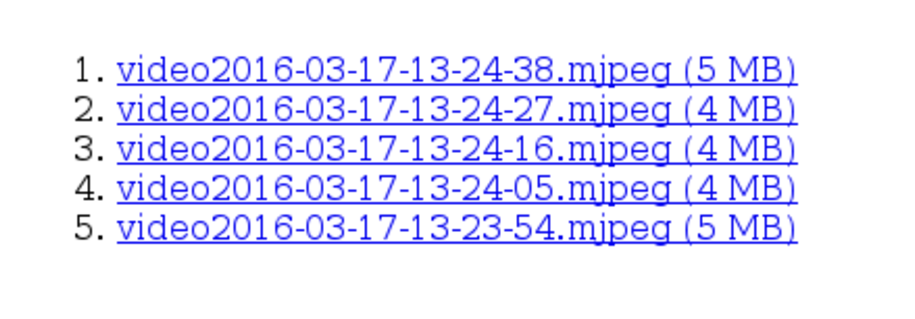
\includegraphics{video-list.eps}}
  \caption{A screenshot of the application's simple interface}
  \label{fig:interface}
\end{figure}

The user interface is coded in \texttt{httpd.c} and \texttt{httpd.h}:

\begin{itemize}
\item \texttt{httpd\_serve}: This is the request dispatcher, or router, if the request path matches a video file name,
then that file is sent to the client for downloading, otherwise the file listing seen in figure \ref{fig:interface} is rendered
\item \texttt{\_httpd\_list\_files} together with \texttt{\_sprint\_video\_list} creates and renders
the set of files available for download, the rendering settings can be configured in the \texttt{config.h} file
\item \texttt{\_httpd\_try\_download} uses the \texttt{sendfile}\footnote{via the \texttt{libmicrohttpd} library}
syscall to optimize the transfer of files between two end-points.
\end{itemize}

I shall note that the video capture part of the application is independent of the \texttt{libmicrohttpd}
library (this can be seen in figure \ref{fig:archdiagram}) and is manually coded in
\texttt{video.c} and \texttt{video.h},
without having any dependencies on a third party library.

This module of the application handles the connection, authentication, retrieval and storage of data
from an IP camera.
 It can be considered the central piece of the experiment.
 The credentials used for authentication to the camera should be stored in the \texttt{credentials.h}
 file (so they should be made available at compile time), similarly to the other parts of the application,
 the address and port on which to connect to the video device cand be configured in the \texttt{config.h} file.

Figure \ref{fig:archdiagram} describes the architecture of the system as a diagram.

\begin{figure}[H]
  \centering
  \fbox{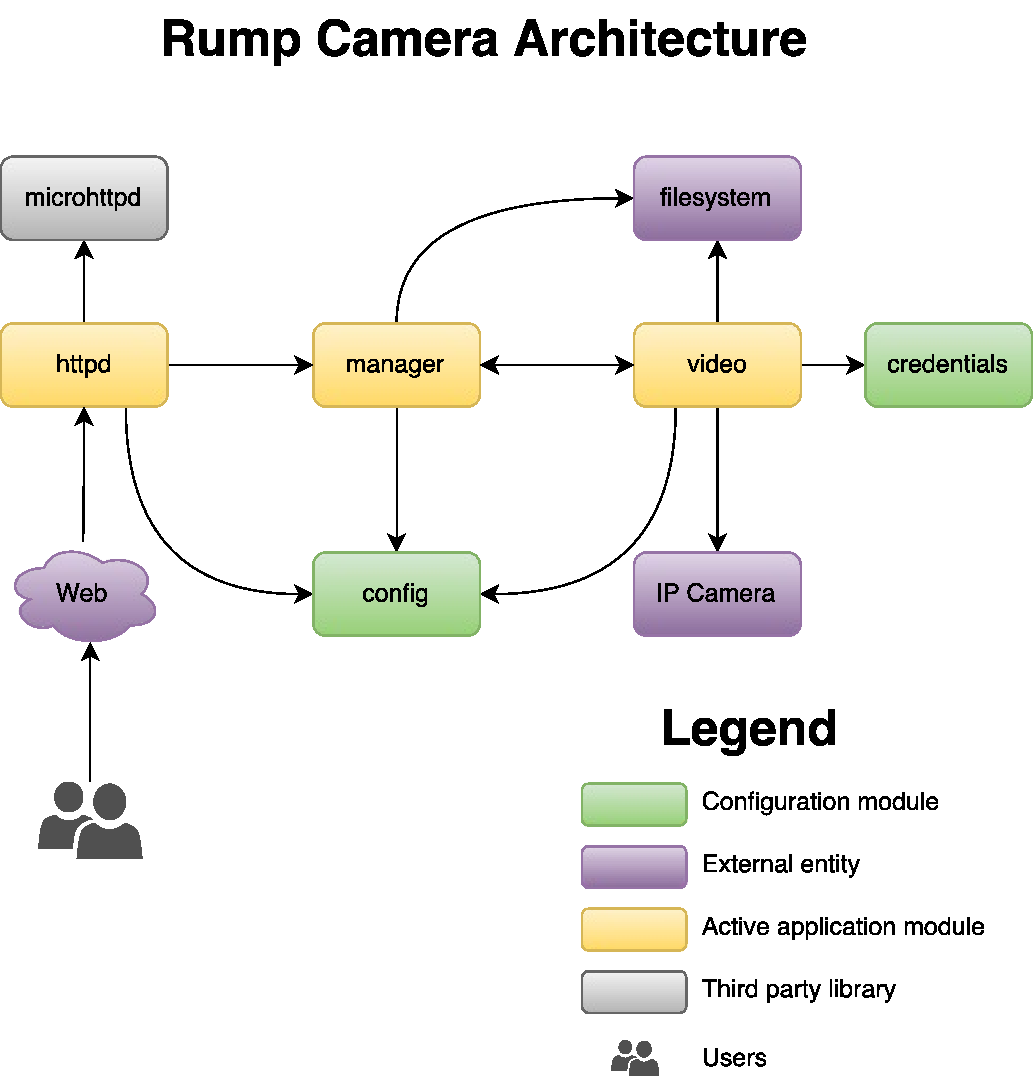
\includegraphics[scale=0.6]{rumpcamera-arch.eps}}
  \caption{The Rump Camera Architecture}
  \label{fig:archdiagram}
\end{figure}

It can be seen that the users have access to the application solely though the web interface, which is implemented by
the \texttt{httpd} module. In turn, this module is supported by the third party library \texttt{libmicrohttpd} which
abstracts away the details of creating, sending and replying to HTTP requests. This library was chosen for its
compactness and because it has an extended test suite. The next module, the \texttt{manager}, is the layer that provides
the order in which the videos were created (for the interface) and decides what video to delete in the event that the
disk becomes full or the maximum number of videos created has been reached.
The \texttt{manager} module is of course in strong relation with the \texttt{video} module, which has the
responsibility to connect to the IP camera (possibly by using authentication) and to store the captured videos on disk.

\section{Future work and conclusions}

Up to this point the main focus of the experiment was simplicity, both in code and in user experience.
So as far as improvements are concerned, the interface of the application can be enhanced by making
it more user friendly, less "brutal". Also the resulting video may be post-processed in order to
include a time-stamp of the capture,
while this post-processing may be made in a parallel fashion (with multiple unikernels working
on different sets of images, similarly to processes in a normal operating system) it would certainly add complexity
into the system.

A downside of static linkage, required by the nature of unikernel applications, are the more
stringent rules that apply when linking a library provided under the GPL license \cite{gpl},
a discussion that quickly escalates into a legal one
\footnote{https://en.wikipedia.org/wiki/GPL\_linking\_exception}. Consequently,
the programmer has to carefully choose his libraries when developing for such an environment where
dynamic linking is not available.

Having a single application that runs on a single (low-power) device, with the unnecessary parts removed out
of the kernel (such as the scheduler) and with only the strictly necessary parts included - such as the drivers),
I believe programmers can write applications that are more environment friendly,
more modular and more robust, being focused on a single, specific task. These modular applications can
then be chained together into a system that resembles software pipe lines or functional composition.

Running these unikernel applications in a virtual environment (like Xen) would also be
beneficial to our surrounding medium since the applications would be started when
needed and stopped at the proper times, thus consuming less energy. \cite{DataCenterEnergyForeCast} \cite{JinWenChen}

This paper successfully demonstrates that surveillance software for IP cameras
(build out of real requirements) can be written to run as a unikernel with minimal footprint and dependencies.
 Such an approach is well suited to this kind of task since the boot-up times
 are much faster due to the reduced code size and, as a consequence, the down-times are small, too.
 Also when security is of concern, the unikernel approach to developing applications can help since
 the attack surface is greatly reduced.

 Of course this approach is not well suited for fast-paced mediums where the software configuration changes often,
 since this would mean too many re-compilations, also this applies for more complex and feature-full software,
 because adding features to a single unikernel application doesn't scale well,
 multiple applications chained together in a computational pipe-line shall be used instead.

 The source code of the application can be freely accessed at: https://github.com/paulbarbu/rump-camera

\begin{thebibliography}{*}\label{Refences}
\bibitem{RumpComparison}
github.com/rumpkernel, \newblock Info: Comparison of rump kernels with similar technologies,
\newblock https://github.com/rumpkernel/wiki/wiki/Info\%3A-Comparison-of-rump-kernels-with-similar-technologies,
\newblock Accessed 15th of March 2016

\vspace{-7pt}
\bibitem{2}
A. Kantee, J. Cormac, \newblock Rump Kernels No OS? No Problem!,
\newblock http://rumpkernel.org/misc/usenix-login-2014/login\_1410\_03\_kantee.pdf,
\newblock October 2014,
\newblock Accessed 15th of March 2016

\vspace{-7pt}
\bibitem{3}
wikipedia.org, \newblock Unikernel,
\newblock https://en.wikipedia.org/wiki/Unikernel,
\newblock Accessed 14th of March 2016

\vspace{-7pt}
\bibitem{DataCenterEnergyForeCast}
Silicon Valley Leadership Group, Accenture, \newblock
Data Centre Energy Forecast Report-Final Report, \newblock July 2008

\vspace{-7pt}
\bibitem{JinWenChen}
Y. Jin, Y. Wen, Q. Chen,
\newblock Energy Efficiency and Server Virtualization in Data Centers: An Empirical Investigation,
\newblock March 2012

\bibitem{gpl}
GNU General Public License, \newblock http://www.gnu.org/licenses/gpl-3.0.en.html,
\newblock Version 3, 29 June 2007,
\newblock Accessed 17th of March 2016

\end{thebibliography}

\vspace*{1cm} {\footnotesize
\begin{tabular*}{16cm}{p{4.2cm}p{4.2cm}p{4.2cm}}
Barbu Paul - Gheorghe & \\
"Lucian Blaga" University of Sibiu & \\
Department of Computer Science and Electrical Engineering & \\
10, Victoriei Bd., Sibiu, 550024, Rom\^ania & \\
ROM\^ANIA & \\
E-mail: \ {\it barbu.paul.gheorghe@gmail.com}&
\end{tabular*}}

\end{document}
